\documentclass[11pt]{article}
\usepackage{hyperref}
\usepackage{graphicx}
\usepackage{amsmath}
\graphicspath{ {./figures/} }

\usepackage[a4paper, left=1.2cm, right=1.2cm, top=1cm, bottom=1cm]{geometry}

\pagenumbering{gobble}

\begin{document}
\title{IVR Coursework 1}
\author{Austin Pan (s1870157) \& Angus Stewart (s1902147)}
\date{\vspace{-5ex}}
\maketitle

\section{Contributions}
Joint State Estimation: Angus Stewart \\
Robot Control: Austin Pan \\
Null-space Control: Austin Pan \& Angus Stewart \\
Github link: \url{https://github.com/Siliconlad/ivr\_assignment}

\section{Joint State Estimation} \label{jse}
\textbf{Note:} for joint 4 we use $\frac{\pi}{3} \sin(\frac{\pi}{20} * t)$ instead of $\frac{\pi}{2} \sin(\frac{\pi}{20} * t)$ as permitted in the follow-up to \href{https://piazza.com/class/kee5t8gp4du6mm?cid=164}{this Piazza post}. \\

\noindent First, we do joint detection on the images from camera 1 \& 2 (in \texttt{image1\_processor} and \texttt{image2\_processor})
\begin{enumerate}
    \item Threshold the HSV image based on the joint colour, find the contour and its center. Take the average of the centres if there's more than one contour. If there are no contours, the joint is hidden.
    \item If the yellow joint has not been detected before, store the center and calculate \texttt{pixel\_to\_meters}.
    \item Shift the centers to be around the yellow center and convert to meters.
\end{enumerate}

\noindent The centers (or \texttt{hidden=True}) are published to \texttt{fusion} to determine the 3D center of each joint. If:
\begin{enumerate}
    \item \textbf{joint centers are received from both images}. The results are combined in the obvious way.
    \item \textbf{one of the joint centers is hidden}. Assume the green joint is hidden in image 1. We find the closest non-hidden object (out of the other joints and the two orange targets) in image 1 to the position $(y_{prev}, z)$ where $y_{prev}$ is the previous $y$ value of the green joint and $z$ is the $z$ value of the green joint from image 2. The new $y$ is the average of the previous $y$ value and the $y$ of the closest object. The $x$ and $z$ values are taken from image 2. The same idea is used for the other objects and for image 2.
    \item \textbf{both of the joint centers are hidden} then return the previous position of the joint
\end{enumerate}

\noindent Finally, in the \texttt{joint\_angles} node we take the 3D positions of the green and red joint from the \texttt{fusion} node and, using the forward kinematics equations, calculate the joint angles.

\begin{center}
    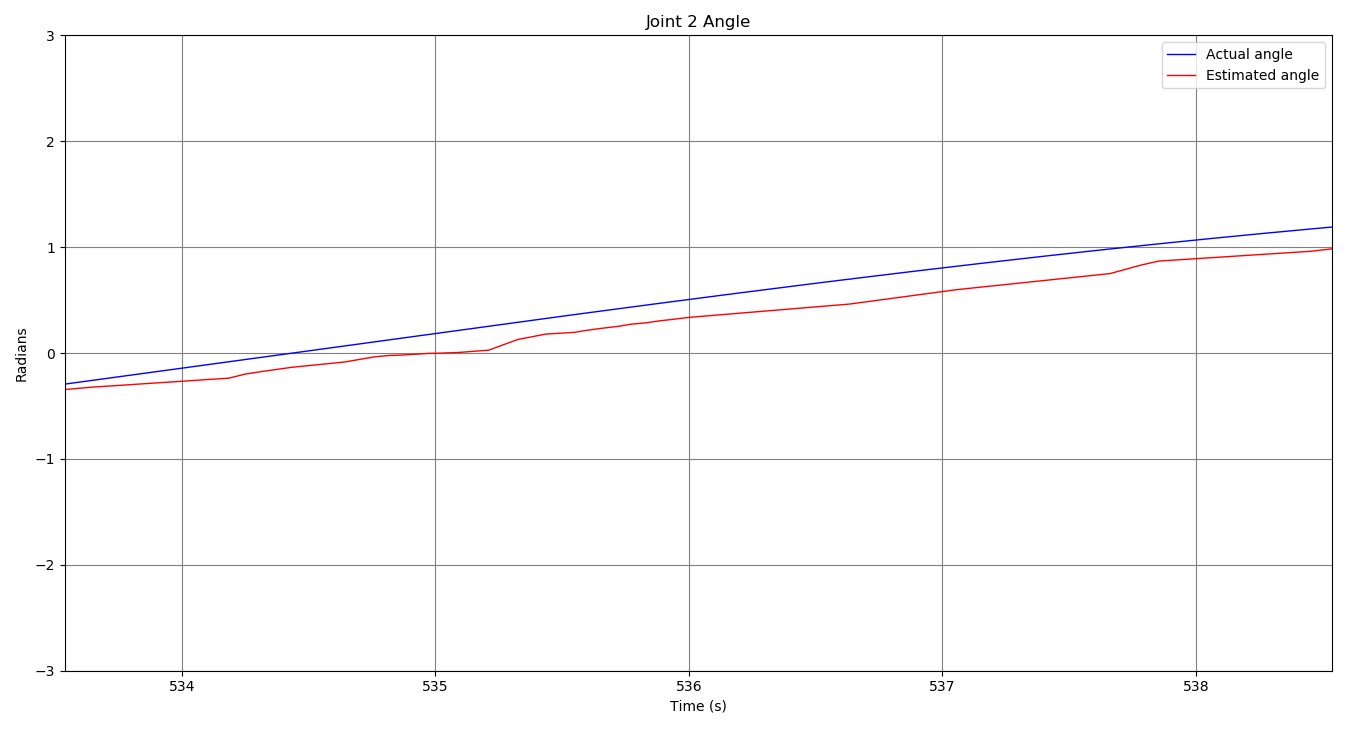
\includegraphics[width=0.7\textwidth]{theta-2} \\
    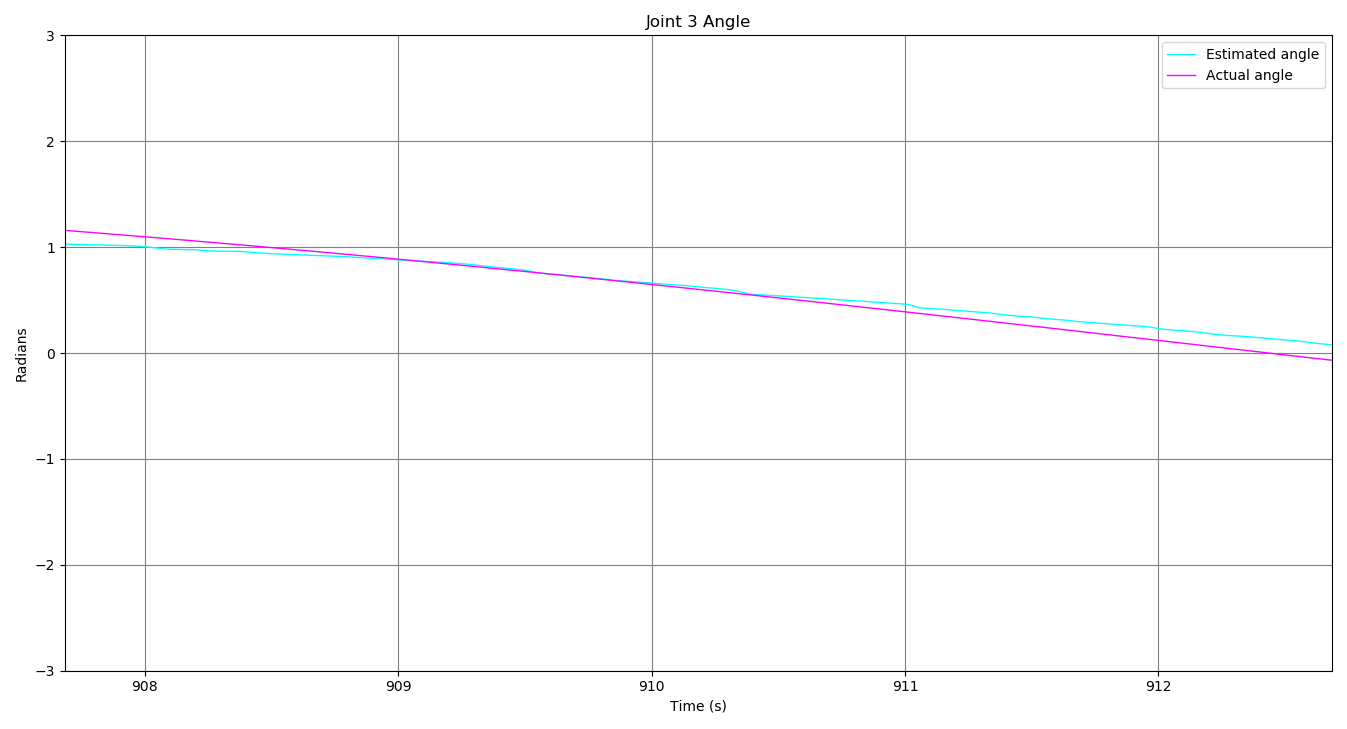
\includegraphics[width=0.7\textwidth]{theta-3} \\
    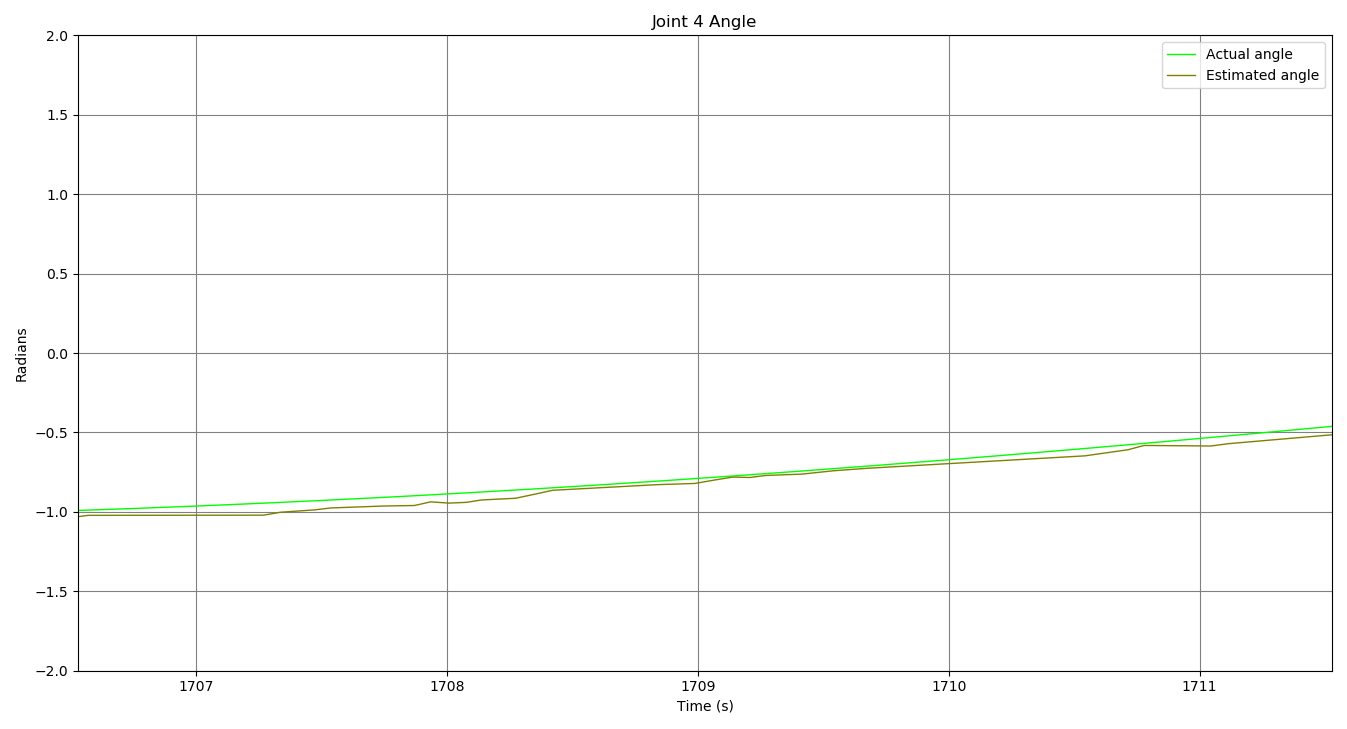
\includegraphics[width=0.7\textwidth]{theta-4} \\
\end{center}

\section{Target Detection}

To get the position of the target sphere, we first detect the sphere in the images from camera 1 and 2:
\begin{enumerate}
	\item Threshold the image in the same way as in section \ref{jse} with the orange color.
	\item Use preselected templates of the target sphere and box and match these to the thresholded image. From this we obtain the centre of the areas matched by each template as well as a numerical measure of how well the template matched the area.
	\item If the centers are within a certain distance of each other, we consider the templates to have matched the same object, hence the object corresponding to the template with the lower score must be hidden.
	\item The centers are then shifted and converted to meters as described in section \ref{jse}.
\end{enumerate}

\noindent The results are then combined to form the 3D position in the same way as described in section \ref{jse}.

\noindent Some sources of error for our position estimate of the target sphere include:
\begin{itemize}
	\item \textbf{Template matching errors} - Because the shape of the sphere is fixed in the template, as the sphere grows or shrinks in size, template matching may find it harder to match the template accurately. This can be seen by the wobbling of the box around the target in the image pop-ups.
	\item \textbf{Perspective error} - Our algorithm assumes that the target is perfectly orthogonal to both cameras at all times. However, this is not realistic (because the target noticeably grows and shrinks) and hence will introduce some amount of error into our estimates.
	\item \textbf{Processing delays} - There may be small errors due to delays from the processing time of our algorithm.
\end{itemize}

\begin{center}
	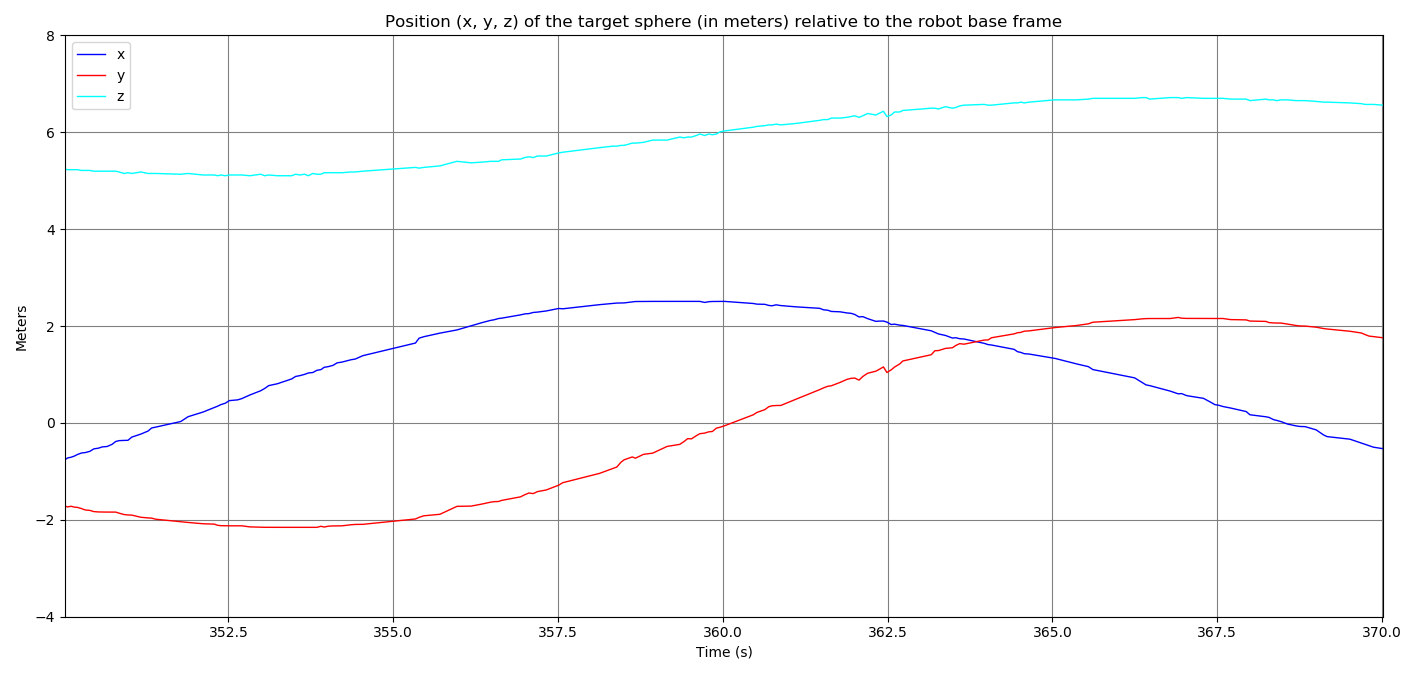
\includegraphics[width=0.7\textwidth]{target-sphere}
\end{center}

\section{Forward Kinematics}

Our forward kinematics equation is given by
\begin{equation*}
\begin{bmatrix}
x_e \\
y_e \\
z_e
\end{bmatrix}
= 
\begin{bmatrix}
3.5s(\theta_1)s(\theta_2)c(\theta_3) + 3.5c(\theta_1)s(\theta_3) + 3s(\theta_1)c(\theta_2)s(\theta_4) + 3s(\theta_1)s(\theta_2)c(\theta_3)c(\theta_4) + 3c(\theta_1)s(\theta_3)c(\theta_4) \\

3.5s(\theta_1)s(\theta_3) - 3.5c(\theta_1)s(\theta_2)c(\theta_3) + 3s(\theta_1)s(\theta_3)c(\theta_4) - 3c(\theta_1)s(\theta_2)c(\theta_3)c(\theta_4) - 3c(\theta_1)c(\theta_2)s(\theta_4)) \\

3.5c(\theta_2)c(\theta_3) + 3c(\theta_2)c(\theta_3)c(\theta_4) - 3s(\theta_2)s(\theta_4) + 2.5
\end{bmatrix}
\end{equation*}


\noindent Below is a table of 10 different configurations of the robot joints and the corresponding estimates of the end-effector position using forward kinematics and computer vision (from section \ref{jse}).

\begin{center}
    \begin{tabular}{ |r|r|r|r||r|r|r|r|r|r|} \hline
        \multicolumn{4}{|c||}{Joint Configuration} & \multicolumn{3}{|c|}{Forward Kinematics} & \multicolumn{3}{|c|}{Computer Vision} \\ \hline
        \multicolumn{1}{|c|}{$\theta_1$} & \multicolumn{1}{|c|}{$\theta_2$} & \multicolumn{1}{|c|}{$\theta_3$} & \multicolumn{1}{|c||}{$\theta_4$} & \multicolumn{1}{|c|}{x} & \multicolumn{1}{|c|}{y} & \multicolumn{1}{|c|}{z} & \multicolumn{1}{|c|}{x} & \multicolumn{1}{|c|}{y} & \multicolumn{1}{|c|}{z} \\ \hline
         0.5 &  0.5 &  0.5 &  0.5 &  4.422 & -1.962 & 6.534 & 5.259 & -2.788 & 6.691 \\
         0.2 &  1.0 &  0.2 &  1.0 &  2.107 & -5.274 & 3.087 & 3.250 & -6.304 & 2.050 \\
         1.0 &  1.0 &  0.4 &  0.4 &  5.934 & -0.911 & 4.634 & 6.575 & -1.315 & 4.196 \\
         0.2 &  0.4 &  0.6 &  0.8 &  3.844 & -3.076 & 5.911 & 4.989 & -4.108 & 5.859 \\
         0.8 &  0.6 &  0.3 &  0.1 &  4.022 & -1.235 & 7.444 & 4.599 & -1.586 & 7.793 \\
        -0.9 &  0.6 & -0.7 &  0.3 & -5.276 &  1.049 & 6.018 & -5.298 & 0.696 & 5.801 \\
        -0.2 & -0.8 & -0.6 &  0.2 & -2.889 &  4.052 & 6.631 & -2.592 & 3.518 & 6.323 \\
         1.2 & -1.0 &  0.7 & -0.3 & -2.779 &  5.481 & 4.385 & -2.425 & 4.834 & 4.351 \\
        -0.3 & -1.2 &  0.8 & -0.7 &  5.290 &  3.035 & 2.162 & 4.602 & 4.834 & 1.354  \\
         1.1 &  1.1 & -1.1 & -1.1 & -1.294 & -4.202 & 5.883 & -1.508 & -4.177 & 5.879 \\ \hline
    \end{tabular}
\end{center}

% INSERT EXPLANATION HERE

\section{Closed-loop Control}

\end{document}
